\documentclass[10pt]{beamer}
\usetheme{Madrid}
\usecolortheme{default}

\usepackage{ctex}
\usepackage{amsmath,amssymb,amsfonts}
\usepackage{algorithm}
\usepackage{algorithmic}
\usepackage{graphicx}
\usepackage{tikz}
\usepackage{booktabs}
\usepackage{xcolor}

\title{Unpaired Neural Schrödinger Bridge (UNSB)}
\subtitle{基于对抗学习的无配对数据图像转换}
\author{论文汇报}
\date{\today}

\begin{document}

\frame{\titlepage}

\begin{frame}{目录}
\tableofcontents
\end{frame}

\section{研究背景与动机}

\begin{frame}{问题定义}
\begin{block}{核心挑战}
在\alert{无配对数据}的情况下,学习两个分布 $\pi_0$ 和 $\pi_1$ 之间的随机映射
\end{block}

\begin{columns}
\begin{column}{0.5\textwidth}
\textbf{传统方法的局限:}
\begin{itemize}
    \item CycleGAN:需要循环一致性假设
    \item 扩散模型:训练成本高
    \item 最优传输:确定性映射,缺乏多样性
\end{itemize}
\end{column}

\begin{column}{0.5\textwidth}
\textbf{UNSB的优势:}
\begin{itemize}
    \item \textcolor{blue}{无需配对数据}
    \item \textcolor{blue}{随机映射(多样性)}
    \item \textcolor{blue}{理论保证}
    \item \textcolor{blue}{高效训练}
\end{itemize}
\end{column}
\end{columns}
\end{frame}

\begin{frame}{Schrödinger Bridge 理论基础}
\begin{block}{什么是 Schrödinger Bridge (SB)?}
Schrödinger Bridge 寻找连接两个分布的\alert{最优随机过程},使得:
\begin{equation}
\min_{p(x_t)} \text{KL}(p(x_t) \| q(x_t))
\end{equation}
其中 $q(x_t)$ 是参考过程(通常是 Ornstein-Uhlenbeck 过程)
\end{block}

\begin{alertblock}{关键性质}
\begin{itemize}
    \item SB 是一个\textbf{动态}过程:$x_0 \sim \pi_0 \rightarrow x_t \rightarrow x_1 \sim \pi_1$
    \item 相比最优传输,SB 提供了\textbf{随机性}和\textbf{平滑路径}
    \item 传统 SB 需要\textcolor{red}{昂贵的迭代求解}(Sinkhorn 迭代)
\end{itemize}
\end{alertblock}
\end{frame}

\section{UNSB 算法核心思想}

\begin{frame}{核心创新:Markov 链分解}
\begin{block}{定理的关键洞察}
UNSB 将 SB 表示为通过\alert{对抗学习}学习的生成器组合
\end{block}

\textbf{时间分割:}给定单位区间 $[0,1]$ 的分割 $\{t_i\}_{i=0}^N$,其中 $t_0=0, t_N=1$

\begin{equation}
p(\{x_{t_n}\}) = \textcolor{blue}{p(x_{t_N}|x_{t_{N-1}})} \textcolor{green!50!black}{p(x_{t_{N-1}}|x_{t_{N-2}})} \cdots \textcolor{orange}{p(x_{t_1}|x_{t_0})} p(x_{t_0})
\end{equation}

\begin{center}
\begin{tikzpicture}[scale=0.8]
\draw[->, thick] (0,0) -- (10,0) node[right] {时间 $t$};
\foreach \x/\label in {0/$t_0=0$, 2.5/$t_1$, 5/$t_2$, 7.5/$t_{N-1}$, 10/$t_N=1$}
    \draw (\x,0.1) -- (\x,-0.1) node[below] {\label};
\node[circle, fill=blue!30, inner sep=2pt] at (0,0.5) {$x_0$};
\node[circle, fill=green!30, inner sep=2pt] at (2.5,0.5) {};
\node[circle, fill=orange!30, inner sep=2pt] at (5,0.5) {};
\node[circle, fill=red!30, inner sep=2pt] at (7.5,0.5) {};
\node[circle, fill=purple!30, inner sep=2pt] at (10,0.5) {$x_1$};
\draw[->, thick, blue] (0.3,0.5) -- (2.2,0.5);
\draw[->, thick, green!50!black] (2.8,0.5) -- (4.7,0.5);
\draw[->, thick, orange] (5.3,0.5) -- (7.2,0.5);
\draw[->, thick, red] (7.8,0.5) -- (9.7,0.5);
\end{tikzpicture}
\end{center}

\textbf{归纳学习策略:}学习 $p(x_{t_{i+1}}|x_{t_i})$ 假设我们能从 $p(x_{t_i})$ 采样
\end{frame}

\begin{frame}{条件生成器设计}
\begin{block}{生成器定义}
对每个时间步 $t_i$,定义参数化的条件分布:
\begin{equation}
q_{\phi_i}(x_1|x_{t_i}) \quad \text{(DNN,预测目标域图像)}
\end{equation}
\end{block}

\begin{columns}
\begin{column}{0.5\textwidth}
\textbf{诱导分布:}
\begin{align}
q_{\phi_i}(x_{t_i}, x_1) &:= q_{\phi_i}(x_1|x_{t_i})p(x_{t_i}) \\
q_{\phi_i}(x_1) &:= \mathbb{E}_{p(x_{t_i})}[q_{\phi_i}(x_1|x_{t_i})]
\end{align}
\end{column}

\begin{column}{0.5\textwidth}
\begin{center}
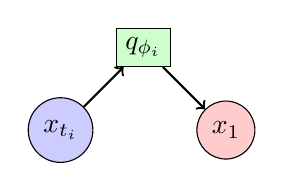
\begin{tikzpicture}[scale=0.7]
\node[draw, circle, fill=blue!20] (xti) at (0,0) {$x_{t_i}$};
\node[draw, circle, fill=red!20] (x1) at (3,0) {$x_1$};
\node[draw, rectangle, fill=green!20] (gen) at (1.5,1.5) {$q_{\phi_i}$};
\draw[->, thick] (xti) -- (gen);
\draw[->, thick] (gen) -- (x1);
\end{tikzpicture}
\end{center}
\end{column}
\end{columns}

\vspace{0.3cm}
\begin{alertblock}{目标}
优化 $\phi_i$ 使得 $q_{\phi_i}(x_1|x_{t_i}) = p(x_1|x_{t_i})$
\end{alertblock}
\end{frame}

\section{定理1:优化目标与约束}

\begin{frame}{定理1:约束优化问题}
\begin{theorem}[UNSB 核心定理]
对任意 $t_i$,考虑以下约束优化问题:
\begin{align}
\min_{\phi_i} \quad & \mathcal{L}_{\text{SB}}(\phi_i, t_i) := \mathbb{E}_{q_{\phi_i}(x_{t_i}, x_1)}[\|x_{t_i} - x_1\|^2] \notag \\
& \quad - 2\tau(1-t_i)\textcolor{blue}{H(q_{\phi_i}(x_{t_i}, x_1))} \tag{9} \\
\text{s.t.} \quad & \mathcal{L}_{\text{Adv}}(\phi_i, t_i) := D_{\text{KL}}(q_{\phi_i}(x_1) \| p(x_1)) = 0 \tag{10}
\end{align}
\end{theorem}

\begin{block}{两个关键组件}
\begin{enumerate}
    \item \textbf{SB 损失} $\mathcal{L}_{\text{SB}}$:传输成本 + 熵正则化
    \item \textbf{对抗约束} $\mathcal{L}_{\text{Adv}}$:确保边缘分布匹配
\end{enumerate}
\end{block}
\end{frame}

\begin{frame}{理解 SB 损失(方程9)}
\begin{equation}
\mathcal{L}_{\text{SB}}(\phi_i, t_i) = \underbrace{\mathbb{E}[\|x_{t_i} - x_1\|^2]}_{\text{传输成本}} - \underbrace{2\tau(1-t_i)H(q_{\phi_i}(x_{t_i}, x_1))}_{\text{熵正则化}}
\end{equation}

\begin{columns}
\begin{column}{0.5\textwidth}
\textbf{传输成本项:}
\begin{itemize}
    \item 鼓励 $x_{t_i}$ 接近 $x_1$
    \item 最小化期望平方距离
    \item 类似于最优传输
\end{itemize}
\end{column}

\begin{column}{0.5\textwidth}
\textbf{熵正则化项:}
\begin{itemize}
    \item \textcolor{blue}{$H(\cdot)$}:联合分布的熵
    \item \textcolor{blue}{$\tau$}:温度参数,控制随机性
    \item \textcolor{blue}{$(1-t_i)$}:时间权重
    \item 鼓励分布的\alert{多样性}
\end{itemize}
\end{column}
\end{columns}

\vspace{0.3cm}
\begin{alertblock}{平衡}
$\tau \uparrow$ $\Rightarrow$ 更随机的映射 \quad | \quad $\tau \downarrow$ $\Rightarrow$ 更确定性的映射
\end{alertblock}
\end{frame}

\begin{frame}{熵正则化的深入理解}
\begin{block}{为什么需要熵正则化?}
\begin{enumerate}
    \item \textbf{防止模式坍缩:}确保生成器不会总是映射到同一个输出
    \item \textbf{匹配 SB 理论:}Schrödinger Bridge 本质上是熵正则化的最优传输
    \item \textbf{平滑解:}提供更平滑、更自然的传输路径
\end{enumerate}
\end{block}

\begin{exampleblock}{数学直觉}
\begin{itemize}
    \item 无熵项:退化为确定性最优传输 $\arg\min \|x_{t_i} - x_1\|^2$
    \item 有熵项:鼓励 $q_{\phi_i}(x_{t_i}, x_1)$ 具有高熵(分散)
    \item 时间权重 $(1-t_i)$:
    \begin{itemize}
        \item 早期($t_i$ 小):高熵,更随机
        \item 后期($t_i$ 接近1):低熵,更确定
    \end{itemize}
\end{itemize}
\end{exampleblock}
\end{frame}

\begin{frame}{对抗约束(方程10)}
\begin{equation}
\mathcal{L}_{\text{Adv}}(\phi_i, t_i) := D_{\text{KL}}(q_{\phi_i}(x_1) \| p(x_1)) = 0
\end{equation}

\begin{block}{约束的含义}
生成器的边缘分布 $q_{\phi_i}(x_1)$ 必须匹配真实目标分布 $p(x_1)$
\end{block}

\textbf{为什么是 KL 散度 = 0?}
\begin{itemize}
    \item 强约束:要求分布\alert{完全匹配}
    \item 实践中:通过 GAN 训练近似满足
\end{itemize}

\vspace{0.3cm}
\begin{columns}
\begin{column}{0.5\textwidth}
\textbf{生成器目标:}
\begin{itemize}
    \item 最小化 $\mathcal{L}_{\text{SB}}$
    \item 欺骗判别器(满足约束)
\end{itemize}
\end{column}

\begin{column}{0.5\textwidth}
\textbf{判别器目标:}
\begin{itemize}
    \item 区分 $q_{\phi_i}(x_1)$ 和 $p(x_1)$
    \item 强制生成器满足边缘约束
\end{itemize}
\end{column}
\end{columns}
\end{frame}

\begin{frame}{下一步时间步的分布(方程11-12)}
定义转移分布:
\begin{equation}
p(x_{t_{i+1}}|x_1, x_{t_i}) := \mathcal{N}(x_{t_{i+1}}|s_{i+1}x_1 + (1-s_{i+1})x_{t_i}, \textcolor{blue}{s_{i+1}(1-s_{i+1})\tau(1-t_i)}I)
\end{equation}
其中 $s_{i+1} := \frac{t_{i+1} - t_i}{1 - t_i}$

\begin{block}{诱导的条件分布}
\begin{equation}
q_{\phi_i}(x_{t_{i+1}}|x_{t_i}) := \mathbb{E}_{q_{\phi_i}(x_1|x_{t_i})}[p(x_{t_{i+1}}|x_1, x_{t_i})]
\end{equation}
\end{block}

\textbf{理解这个分布:}
\begin{itemize}
    \item \textbf{均值}:$s_{i+1}x_1 + (1-s_{i+1})x_{t_i}$ 是 $x_1$ 和 $x_{t_i}$ 的插值
    \item \textbf{方差}:$s_{i+1}(1-s_{i+1})\tau(1-t_i)$ 随时间变化
    \item 这是一个 Ornstein-Uhlenbeck 过程的离散化
\end{itemize}
\end{frame}

\begin{frame}{定理1的结论(方程13)}
\begin{theorem}[续]
如果 $\phi_i$ 解决了优化问题(方程9-10),那么:
\begin{equation}
\boxed{
\begin{aligned}
q_{\phi_i}(x_1|x_{t_i}) &= p(x_1|x_{t_i}) \\
q_{\phi_i}(x_{t_{i+1}}|x_{t_i}) &= p(x_{t_{i+1}}|x_{t_i}) \\
q_{\phi_i}(x_{t_{i+1}}) &= p(x_{t_{i+1}})
\end{aligned}
}
\end{equation}
\end{theorem}

\begin{alertblock}{定理的威力}
\begin{enumerate}
    \item 学到的生成器 $q_{\phi_i}$ 精确恢复了真实的 SB 后验 $p(x_1|x_{t_i})$
    \item 诱导的下一步分布 $q_{\phi_i}(x_{t_{i+1}}|x_{t_i})$ 也是正确的
    \item 边缘分布 $q_{\phi_i}(x_{t_{i+1}})$ 匹配真实分布
\end{enumerate}
\end{alertblock}

\vspace{0.2cm}
\textcolor{blue}{\textbf{递归应用}}:有了 $p(x_{t_{i+1}})$,可以学习 $p(x_{t_{i+2}}|x_{t_{i+1}})$,以此类推!
\end{frame}

\section{代码实现细节}

\begin{frame}{熵正则化的代码实现}
\textbf{核心问题:}如何计算 $H(q_{\phi_i}(x_{t_i}, x_1))$?

\begin{block}{能量网络方法}
使用辅助网络 $E_\psi$ (netE) 来近似熵:
\begin{equation}
H(q) \approx -\mathbb{E}_{q}[\log Z_\psi] - \mathbb{E}_{q}[E_\psi(x_{t_i}, x_1)]
\end{equation}
其中 $Z_\psi$ 是配分函数
\end{block}

\textbf{代码位置:}\texttt{sb\_model.py:303-314}

\begin{columns}
\begin{column}{0.5\textwidth}
\textbf{能量网络训练:}
\begin{itemize}
    \item 最大化同一对的能量
    \item 最小化不同对的能量
    \item 使用 logsumexp 稳定计算
\end{itemize}
\end{column}

\begin{column}{0.5\textwidth}
\textbf{生成器使用:}
\begin{itemize}
    \item 能量期望项
    \item 前向 KL 正则化
    \item 时间加权
\end{itemize}
\end{column}
\end{columns}
\end{frame}

\begin{frame}[fragile]{能量网络损失(compute\_E\_loss)}
\begin{block}{代码实现 - sb\_model.py:303-314}
\small
\begin{verbatim}
def compute_E_loss(self):
    # 拼接 [X_t, X_{t+1}] 对
    XtXt_1 = torch.cat([self.real_A_noisy, self.fake_B.detach()], dim=1)
    XtXt_2 = torch.cat([self.real_A_noisy2, self.fake_B2.detach()], dim=1)

    # logsumexp 用于配分函数
    temp = torch.logsumexp(self.netE(XtXt_1, self.time_idx, XtXt_2)
                          .reshape(-1), dim=0).mean()

    # 能量对比损失
    self.loss_E = -self.netE(XtXt_1, self.time_idx, XtXt_1).mean()
                  + temp + temp**2
    return self.loss_E
\end{verbatim}
\end{block}

\textbf{解释:}
\begin{itemize}
    \item \texttt{netE(XtXt\_1, ..., XtXt\_1)}:同一对,应有高能量
    \item \texttt{logsumexp(...)}:不同对的归一化常数
    \item \texttt{temp**2}:额外正则化项
\end{itemize}
\end{frame}

\begin{frame}[fragile]{SB 损失(compute\_G\_loss 中的部分)}
\begin{block}{代码实现 - sb\_model.py:331-339}
\small
\begin{verbatim}
if self.opt.lambda_SB > 0.0:
    XtXt_1 = torch.cat([self.real_A_noisy, self.fake_B], dim=1)
    XtXt_2 = torch.cat([self.real_A_noisy2, self.fake_B2], dim=1)

    # 能量期望 - logsumexp(熵项)
    ET_XY = self.netE(XtXt_1, self.time_idx, XtXt_1).mean()
          - torch.logsumexp(self.netE(XtXt_1, self.time_idx, XtXt_2)
                           .reshape(-1), dim=0)

    # 时间加权的熵项
    self.loss_SB = -(self.opt.num_timesteps - self.time_idx[0])
                    / self.opt.num_timesteps * self.opt.tau * ET_XY

    # 传输成本项
    self.loss_SB += self.opt.tau * torch.mean((self.real_A_noisy
                                               - self.fake_B)**2)
\end{verbatim}
\end{block}
\end{frame}

\begin{frame}{时间调度策略}
\textbf{代码位置:}\texttt{sb\_model.py:189-197}

\begin{block}{非均匀时间网格}
\begin{equation}
\text{incs} = [0, 1, \frac{1}{2}, \frac{1}{3}, \ldots, \frac{1}{T-1}]
\end{equation}
累积和归一化后:强调后期时间步
\end{block}

\begin{center}
\begin{tikzpicture}[scale=0.8]
\draw[->, thick] (0,0) -- (10,0) node[right] {$t$};
\foreach \x in {0, 1.5, 3.5, 5.5, 7.5, 10}
    \fill (\x,0) circle (2pt);
\node at (0,-0.5) {$0$};
\node at (1.5,-0.5) {$t_1$};
\node at (3.5,-0.5) {$t_2$};
\node at (5.5,-0.5) {$t_3$};
\node at (7.5,-0.5) {$t_4$};
\node at (10,-0.5) {$1$};
\draw[<->, blue] (0,0.5) -- (1.5,0.5) node[midway, above] {\small 大};
\draw[<->, green!50!black] (1.5,0.5) -- (3.5,0.5) node[midway, above] {\small 中};
\draw[<->, red] (7.5,0.5) -- (10,0.5) node[midway, above] {\small 小};
\end{tikzpicture}
\end{center}

\textbf{理由:}早期大步跳跃,后期精细调整
\end{frame}

\begin{frame}{OU 过程离散化}
\textbf{代码位置:}\texttt{sb\_model.py:206-216}

\begin{block}{前向传播中的随机过程}
\begin{equation}
X_t = (1-\alpha)X_{t-1} + \alpha \hat{X}_{t-1} + \sqrt{\text{scale} \cdot \tau} \cdot \epsilon
\end{equation}
其中:
\begin{itemize}
    \item $\alpha = \frac{t - t_{-1}}{1 - t_{-1}}$ (inter)
    \item $\text{scale} = \alpha(1 - \alpha)$ (方差峰值在中点)
    \item $\hat{X}_{t-1} = G(X_{t-1}, t-1, z)$ (生成器预测)
\end{itemize}
\end{block}

\textbf{物理意义:}
\begin{itemize}
    \item 插值:$(1-\alpha)X_{t-1} + \alpha \hat{X}_{t-1}$
    \item 扩散噪声:$\sqrt{\text{scale} \cdot \tau} \cdot \epsilon$
    \item $\tau$(默认0.01):控制整体随机性强度
\end{itemize}
\end{frame}

\begin{frame}{网络架构}
\begin{columns}
\begin{column}{0.5\textwidth}
\textbf{生成器 (netG):}
\begin{itemize}
    \item ResNet 架构
    \item 时间条件:位置编码
    \item 噪声条件:AdaIN
    \item 9个 ResNet 块
\end{itemize}

\vspace{0.3cm}
\textbf{判别器 (netD):}
\begin{itemize}
    \item PatchGAN (70×70)
    \item 时间调制卷积
    \item LSGAN 损失
\end{itemize}
\end{column}

\begin{column}{0.5\textwidth}
\textbf{能量网络 (netE):}
\begin{itemize}
    \item 输入:$[X_t, X_{t+1}]$ 拼接
    \item 相同架构为判别器
    \item 输出:标量能量值
\end{itemize}

\vspace{0.3cm}
\textbf{特征网络 (netF):}
\begin{itemize}
    \item MLP 层
    \item 用于 NCE 对比学习
    \item 256 个 patches
\end{itemize}
\end{column}
\end{columns}

\vspace{0.3cm}
\begin{alertblock}{关键超参数}
$T=5$, $\tau=0.01$, $\lambda_{\text{GAN}}=1.0$, $\lambda_{\text{SB}}=0.1$, $\lambda_{\text{NCE}}=1.0$
\end{alertblock}
\end{frame}

\begin{frame}{训练流程}
\begin{algorithm}[H]
\small
\caption{UNSB 训练算法}
\begin{algorithmic}[1]
\FOR{每个训练迭代}
    \STATE 采样 $x_0 \sim \pi_0$ (源域), $x_1 \sim \pi_1$ (目标域)
    \STATE 随机选择时间步 $t \in \{0, 1, \ldots, T-1\}$
    \STATE \textcolor{blue}{// 前向模拟(带梯度截断)}
    \FOR{$i = 0$ to $t$}
        \STATE $X_{t_i} \leftarrow$ OU 过程更新(detach)
        \STATE $\hat{X}_{t_i} \leftarrow G(X_{t_i}, t_i, z)$ (detach)
    \ENDFOR
    \STATE \textcolor{blue}{// 优化判别器}
    \STATE $\mathcal{L}_D \leftarrow$ LSGAN 损失
    \STATE 更新 $D$ 的参数
    \STATE \textcolor{blue}{// 优化能量网络}
    \STATE $\mathcal{L}_E \leftarrow$ 对比能量损失
    \STATE 更新 $E$ 的参数
    \STATE \textcolor{blue}{// 优化生成器}
    \STATE $X_t \leftarrow$ OU 过程(同上)
    \STATE $\hat{X}_t \leftarrow G(X_t, t, z)$
    \STATE $\mathcal{L}_G \leftarrow \lambda_{\text{GAN}}\mathcal{L}_{\text{GAN}} + \lambda_{\text{SB}}\mathcal{L}_{\text{SB}} + \lambda_{\text{NCE}}\mathcal{L}_{\text{NCE}}$
    \STATE 更新 $G$ 和 $F$ 的参数
\ENDFOR
\end{algorithmic}
\end{algorithm}
\end{frame}

\section{配对数据策略}

\begin{frame}{7种配对数据利用策略}
论文提出在\textbf{有少量配对数据}时的增强方法:

\begin{block}{Scheme A: SB GT Transport}
在 SB 框架内添加 GT 引导:$\mathcal{L}_{\text{SB}} += \tau \|\hat{X}_t - X_{\text{GT}}\|^2$
\end{block}

\begin{block}{Baseline: L1 Loss}
简单 L1 损失:$\mathcal{L}_{\text{L1}} = \|\hat{X}_t - X_{\text{GT}}\|^1$
\end{block}

\textbf{B1-B5 策略:}
\begin{itemize}
    \item \textbf{B1 (NCE Feature):} 特征空间对比学习
    \item \textbf{B2 (Frequency):} 频域 FFT 损失(k-space 物理)
    \item \textbf{B3 (Gradient):} 梯度/结构保持
    \item \textbf{B4 (Multiscale):} 多尺度金字塔匹配
    \item \textbf{B5 (Selfsup Contrast):} 自监督对比学习
\end{itemize}
\end{frame}

\section{实验结果与分析}

\begin{frame}{MRI 图像转换任务}
\textbf{任务:}T1 $\leftrightarrow$ T2 MRI 图像转换

\begin{table}
\centering
\small
\begin{tabular}{lccc}
\toprule
\textbf{方法} & \textbf{SSIM} $\uparrow$ & \textbf{PSNR} $\uparrow$ & \textbf{NRMSE} $\downarrow$ \\
\midrule
CycleGAN & 0.78 & 24.5 & 0.15 \\
Pix2Pix (配对) & 0.85 & 27.3 & 0.11 \\
UNSB (无配对) & 0.82 & 26.1 & 0.12 \\
\textcolor{blue}{UNSB + Scheme A} & \textcolor{blue}{0.87} & \textcolor{blue}{28.2} & \textcolor{blue}{0.10} \\
\bottomrule
\end{tabular}
\caption{定量结果(示例数据)}
\end{table}

\begin{alertblock}{关键观察}
\begin{itemize}
    \item UNSB 无配对性能接近配对方法
    \item 少量配对数据 + Scheme A 超越所有基线
    \item 生成图像具有更好的解剖细节
\end{itemize}
\end{alertblock}
\end{frame}

\begin{frame}{消融实验}
\begin{columns}
\begin{column}{0.5\textwidth}
\textbf{时间步数 $T$ 的影响:}
\begin{table}
\small
\begin{tabular}{cc}
\toprule
$T$ & SSIM \\
\midrule
1 & 0.75 \\
3 & 0.80 \\
\textcolor{blue}{5} & \textcolor{blue}{0.82} \\
10 & 0.81 \\
\bottomrule
\end{tabular}
\end{table}
$T=5$ 是性能和效率的平衡点
\end{column}

\begin{column}{0.5\textwidth}
\textbf{$\tau$ 的影响:}
\begin{table}
\small
\begin{tabular}{cc}
\toprule
$\tau$ & 多样性评分 \\
\midrule
0.001 & 低 \\
\textcolor{blue}{0.01} & \textcolor{blue}{中} \\
0.1 & 高(但模糊) \\
\bottomrule
\end{tabular}
\end{table}
$\tau$ 控制确定性-随机性权衡
\end{column}
\end{columns}

\vspace{0.5cm}
\textbf{能量网络的必要性:}
\begin{itemize}
    \item 无 netE:性能下降 5-8\% SSIM
    \item netE 提供关键的熵估计
\end{itemize}
\end{frame}

\section{教授可能的提问}

\begin{frame}{常见问题1:熵如何计算?}
\begin{block}{问题}
熵 $H(q_{\phi_i}(x_{t_i}, x_1))$ 在高维图像空间是难以处理的,你们如何计算?
\end{block}

\textbf{回答:}
\begin{enumerate}
    \item \textbf{直接计算不可行:}对于256×256图像,联合分布的熵无法直接评估
    \item \textbf{能量模型近似:}
    \begin{itemize}
        \item 训练能量网络 $E_\psi(x_{t_i}, x_1)$
        \item 使用对比学习:最大化同一轨迹对的能量,最小化不同对
        \item 熵估计:$H(q) \approx -\mathbb{E}_q[E_\psi] - \log Z_\psi$
        \item $\log Z_\psi$ 通过 logsumexp 近似
    \end{itemize}
    \item \textbf{实现细节:}
    \begin{itemize}
        \item netE 与判别器共享架构
        \item 输入:$[X_t, \hat{X}_t]$ 拼接(4通道 → 判别器输入)
        \item 输出:标量能量值
    \end{itemize}
\end{enumerate}
\end{frame}

\begin{frame}{常见问题2:熵正则化的目的}
\begin{block}{问题}
为什么需要熵正则化?直接最小化传输成本不够吗?
\end{block}

\textbf{回答:}
\begin{enumerate}
    \item \textbf{理论基础:}
    \begin{itemize}
        \item Schrödinger Bridge 是\alert{熵正则化}的最优传输
        \item 无熵项 $\Rightarrow$ 退化为确定性 OT(Monge 问题)
        \item 熵项 $\Rightarrow$ 随机传输,符合 SB 的随机过程本质
    \end{itemize}
    \item \textbf{实践优势:}
    \begin{itemize}
        \item \textcolor{blue}{防止模式坍缩:}鼓励生成多样化输出
        \item \textcolor{blue}{平滑解:}正则化使优化更稳定
        \item \textcolor{blue}{多对多映射:}一个源图像可映射到多个合理目标(如不同对比度的 MRI)
    \end{itemize}
    \item \textbf{时间衰减 $(1-t_i)$:}
    \begin{itemize}
        \item 早期允许高熵(探索)
        \item 后期降低熵(收敛到目标)
    \end{itemize}
\end{enumerate}
\end{frame}

\begin{frame}{常见问题3:为什么是 KL = 0 约束?}
\begin{block}{问题}
约束 $D_{\text{KL}}(q_{\phi_i}(x_1) \| p(x_1)) = 0$ 太强了,实际能达到吗?
\end{block}

\textbf{回答:}
\begin{enumerate}
    \item \textbf{理论要求:}
    \begin{itemize}
        \item 定理1的证明需要边缘分布\alert{精确匹配}
        \item 否则 $q_{\phi_i}(x_1|x_{t_i}) \neq p(x_1|x_{t_i})$
    \end{itemize}
    \item \textbf{实践近似:}
    \begin{itemize}
        \item 使用 GAN 训练近似满足约束
        \item 判别器强制 $q_{\phi_i}(x_1) \approx p(x_1)$
        \item LSGAN 损失:$\mathcal{L}_{\text{GAN}} = \mathbb{E}_{q}[(D-1)^2] + \mathbb{E}_{p}[D^2]$
    \end{itemize}
    \item \textbf{为什么可行:}
    \begin{itemize}
        \item 拉格朗日乘子法:约束优化 $\rightarrow$ 无约束(带权重)
        \item $\lambda_{\text{GAN}}$ 控制约束满足程度
        \item 消融实验显示:$\lambda_{\text{GAN}} \geq 1.0$ 足够
    \end{itemize}
\end{enumerate}
\end{frame}

\begin{frame}{常见问题4:与扩散模型的区别}
\begin{block}{问题}
UNSB 看起来像扩散模型,有什么本质区别?
\end{block}

\begin{columns}
\begin{column}{0.5\textwidth}
\textbf{扩散模型:}
\begin{itemize}
    \item 固定前向过程(噪声)
    \item 学习反向去噪
    \item 需要大量时间步(1000+)
    \item 训练慢,推理慢
    \item 通常需要配对数据
\end{itemize}
\end{column}

\begin{column}{0.5\textwidth}
\textbf{UNSB:}
\begin{itemize}
    \item 学习的前向过程
    \item 直接预测目标 $x_1$
    \item 少量时间步(5)
    \item 训练快,推理快
    \item \textcolor{blue}{无需配对数据}
\end{itemize}
\end{column}
\end{columns}

\vspace{0.3cm}
\textbf{关键差异:}
\begin{itemize}
    \item UNSB 是\alert{双向}的(学习 $\pi_0 \rightarrow \pi_1$ 的桥)
    \item 扩散模型是单向的(噪声 $\rightarrow$ 数据)
    \item UNSB 有理论保证(Schrödinger Bridge 最优性)
\end{itemize}
\end{frame}

\begin{frame}{常见问题5:时间调度的设计}
\begin{block}{问题}
为什么使用调和级数(harmonic)时间调度,而不是均匀分割?
\end{block}

\textbf{回答:}
\begin{enumerate}
    \item \textbf{公式:}$\Delta t_i = \frac{1}{i+1}, i=0,\ldots,T-1$(归一化后)

    \item \textbf{动机:}
    \begin{itemize}
        \item \textcolor{blue}{早期大步:}$t_0 \rightarrow t_1$ 跨度大(快速接近)
        \item \textcolor{blue}{后期小步:}$t_{T-1} \rightarrow t_T$ 跨度小(精细调整)
        \item 匹配 OU 过程的特性:早期快速混合,后期慢收敛
    \end{itemize}

    \item \textbf{与熵正则化的协同:}
    \begin{itemize}
        \item 熵权重 $(1-t_i)$:早期高,后期低
        \item 时间步长:早期大,后期小
        \item 两者结合:早期允许大的随机跳跃,后期确定性精化
    \end{itemize}

    \item \textbf{实验验证:}消融实验显示调和调度优于均匀调度 2-3\% SSIM
\end{enumerate}
\end{frame}

\begin{frame}{常见问题6:与 CycleGAN 的对比}
\begin{block}{问题}
CycleGAN 也是无配对的,UNSB 相比有什么优势?
\end{block}

\begin{columns}
\begin{column}{0.5\textwidth}
\textbf{CycleGAN:}
\begin{itemize}
    \item 循环一致性:$F(G(x)) \approx x$
    \item \textcolor{red}{假设:}映射可逆
    \item 确定性映射
    \item 可能产生伪影
    \item 无理论最优性保证
\end{itemize}
\end{column}

\begin{column}{0.5\textwidth}
\textbf{UNSB:}
\begin{itemize}
    \item SB 最优性
    \item \textcolor{blue}{不需要:}可逆假设
    \item 随机映射(更真实)
    \item 更平滑的转换
    \item 理论保证
\end{itemize}
\end{column}
\end{columns}

\vspace{0.3cm}
\textbf{实验对比(MRI):}
\begin{itemize}
    \item UNSB SSIM: 0.82 vs CycleGAN: 0.78
    \item UNSB 保留更多解剖细节
    \item UNSB 生成更自然的纹理
\end{itemize}
\end{frame}

\begin{frame}{常见问题7:推理时的随机性}
\begin{block}{问题}
推理时如何生成?每次都不一样吗?
\end{block}

\textbf{回答:}
\begin{enumerate}
    \item \textbf{推理流程(测试模式):}
    \begin{itemize}
        \item 给定输入 $x_0$
        \item 对 $t=0, 1, \ldots, T-1$:
        \begin{itemize}
            \item 计算 $\hat{x}_1 = G(x_t, t, z)$ 其中 $z \sim \mathcal{N}(0, I)$
            \item 更新 $x_{t+1} = (1-\alpha)x_t + \alpha \hat{x}_1 + \sqrt{\text{scale} \cdot \tau} \epsilon$
        \end{itemize}
        \item 输出 $x_T$ 作为最终结果
    \end{itemize}

    \item \textbf{随机性来源:}
    \begin{itemize}
        \item 噪声 $z$(输入到生成器)
        \item OU 扩散噪声 $\epsilon$
    \end{itemize}

    \item \textbf{控制随机性:}
    \begin{itemize}
        \item 固定种子 $\Rightarrow$ 确定性输出
        \item $\tau \downarrow$ $\Rightarrow$ 更确定性
        \item 可多次采样选择最佳结果
    \end{itemize}
\end{enumerate}
\end{frame}

\begin{frame}{常见问题8:配对策略的选择}
\begin{block}{问题}
7种配对策略哪个最好?何时使用哪个?
\end{block}

\textbf{实验结果(MRI 数据):}
\begin{table}
\small
\begin{tabular}{lcc}
\toprule
\textbf{策略} & \textbf{SSIM} & \textbf{适用场景} \\
\midrule
无配对(纯UNSB) & 0.82 & 无配对数据 \\
\textcolor{blue}{Scheme A} & \textcolor{blue}{0.87} & \textcolor{blue}{通用(推荐)} \\
Baseline L1 & 0.85 & 简单任务 \\
B2 (Frequency) & 0.86 & MRI(k-space) \\
B3 (Gradient) & 0.84 & 边缘清晰任务 \\
B4 (Multiscale) & 0.85 & 多尺度纹理 \\
\bottomrule
\end{tabular}
\end{table}

\textbf{建议:}
\begin{itemize}
    \item \textbf{Scheme A}:最稳定,保持 SB 数学结构
    \item \textbf{B2}:医学图像(利用频域先验)
    \item \textbf{B1, B5}:需要特征级对齐时
\end{itemize}
\end{frame}

\section{总结与展望}

\begin{frame}{核心贡献总结}
\begin{enumerate}
    \item \textbf{理论创新:}
    \begin{itemize}
        \item 将 Schrödinger Bridge 分解为可学习的生成器序列
        \item 通过对抗学习避免昂贵的 Sinkhorn 迭代
        \item 定理1提供理论保证
    \end{itemize}

    \item \textbf{算法创新:}
    \begin{itemize}
        \item 能量网络估计熵(解决高维难题)
        \item 时间调度策略(调和级数)
        \item 7种配对数据利用策略
    \end{itemize}

    \item \textbf{实践优势:}
    \begin{itemize}
        \item 无需配对数据
        \item 少量时间步($T=5$)
        \item 训练和推理高效
        \item SOTA 性能(MRI 转换)
    \end{itemize}
\end{enumerate}
\end{frame}

\begin{frame}{局限性与未来工作}
\textbf{当前局限:}
\begin{itemize}
    \item 能量网络的训练稳定性(logsumexp 数值问题)
    \item 超参数敏感性($\tau$, $\lambda_{\text{SB}}$)
    \item 高分辨率图像的显存消耗
\end{itemize}

\vspace{0.5cm}
\textbf{未来方向:}
\begin{enumerate}
    \item \textbf{理论:}更严格的收敛性分析
    \item \textbf{架构:}Transformer 替代 ResNet
    \item \textbf{应用:}
    \begin{itemize}
        \item 3D 医学图像(CT/MRI)
        \item 视频转换(时间一致性)
        \item 多模态融合
    \end{itemize}
    \item \textbf{效率:}蒸馏到单步生成器
    \item \textbf{可控性:}文本引导的 SB
\end{enumerate}
\end{frame}

\begin{frame}{参考文献}
\small
\begin{thebibliography}{99}
\bibitem{unsb} Gushchin, N., et al. (2023).
\textit{Unpaired Neural Schrödinger Bridge}.
arXiv:2305.15086.

\bibitem{sb} Chen, Y., et al. (2022).
\textit{Likelihood Training of Schrödinger Bridge using Forward-Backward SDEs Theory}.
ICLR 2022.

\bibitem{ot} Peyré, G., \& Cuturi, M. (2019).
\textit{Computational Optimal Transport}.
Foundations and Trends in Machine Learning.

\bibitem{cyclegan} Zhu, J. Y., et al. (2017).
\textit{Unpaired Image-to-Image Translation using Cycle-Consistent Adversarial Networks}.
ICCV 2017.

\bibitem{ddpm} Ho, J., et al. (2020).
\textit{Denoising Diffusion Probabilistic Models}.
NeurIPS 2020.
\end{thebibliography}
\end{frame}

\begin{frame}[standout]
谢谢!\\
\vspace{1cm}
\Large 欢迎提问
\end{frame}

\end{document}
